\documentclass[a4paper,12pt]{scrartcl}
\usepackage[utf8x]{inputenc}
\usepackage[T1]{fontenc} % avec T1 comme option  d'encodage c'est ben mieux, surtout pour taper du français.
%\usepackage{lmodern,textcomp} % fortement conseillé pour les pdf. On peut mettre autre chose : kpfonts, fourier,...
\usepackage[french]{babel} %Sans ça les guillemets, amarchpo
\usepackage{amsmath}
\usepackage{multicol}
\usepackage{amssymb}
\usepackage{tkz-tab}
\usepackage{exercice_sheet}

%\trait
%\section*{}
%\exo{}
%\question{}
%\subquestion{}

\date{}


% Title Page
\title{Devoir maison 1, CG-2}

\author{Mathématiques}

\begin{document}

\maketitle

\exo{Équations, inéquations}

Résoudre les équations et inéquations suivantes.

\begin{multicols}{2}

\question{}
$\ln(x+1) + \ln(x-2) = \ln(18)$

\question{}
$2e^{2t} + 9e^t = 5$

\question{}
$2e^{2t} - 9e^t + 4 = 0$

\question{}
$\ln(x^4) < 12$

\end{multicols}

\exo{Suites numériques}

On compare l'évolution de la fréquentation de 2 écoles A et B. En 2015, l'école A compte 310 élèves et l'école B en compte 280. On fait l'hypothèse que chaque année, l'effectif de l'école A augmente de 10 élèves tandis que celui de l'école B augmente de 5\%.

\question{Justifier que le nombre d'élèves de l'école B pour l'année $2015+n$ peut être modélisé par une suite géométrique $(b_n)$ dont on précisera le premier terme $b_0$ et la raison $q$.}

\question{La capacité de l'école B est de 450 élèves. Pourra-t-elle accueillir tous les élèves prévus par le modèle jusqu'en 2025?}

\question{}
Dans le tableur ci-dessous, quelle formule dois-je écrire dans la cellule C3 pour calculer l'effectif de l'école A? 

Même question pour la cellule D3, qui concerne l'école B.

Que faire pour que les colonnes entières soient calculées sans avoir à taper la formule dans chaque case de chaque colonne?

\begin{center}
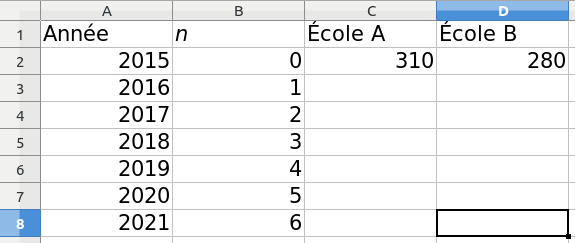
\includegraphics[width=0.5\textwidth]{pics/1.png}
\end{center}

\exo{Étude d'une fonction}

On considère la fonction $f$ définie sur $[0;+\infty[$ par:

$$f(x) = 0.4 e^{0.3x}$$

On désigne par $C$ sa courbe représentative dans un repère orthogonal et par $f'$ sa fonction dérivée. Unités graphiques: 1cm pour une unité sur l'axe des abscisses et 1cm pour 2 unités sur l'axe des ordonnées.

\question{Étudier la limite\footnote{Les limites ne sont pas au programme pour les suites mais le sont pour les fonctions.} de $f$ en $+\infty$.}

\question{Étude de la fonction}

\subquestion{Calculer $f'(x)$}

\subquestion{Étudier le signe de $f'(x)$ et donner le tableau de variation de $f$ sur $[0;+\infty[$.}

\subquestion{Tracer $C$. Une feuille à petit carreaux fera parfaitement l'affaire.}

\trait

\begin{center}
Fin.
\end{center}

\end{document}
